\begin{figure}[H]
\centering
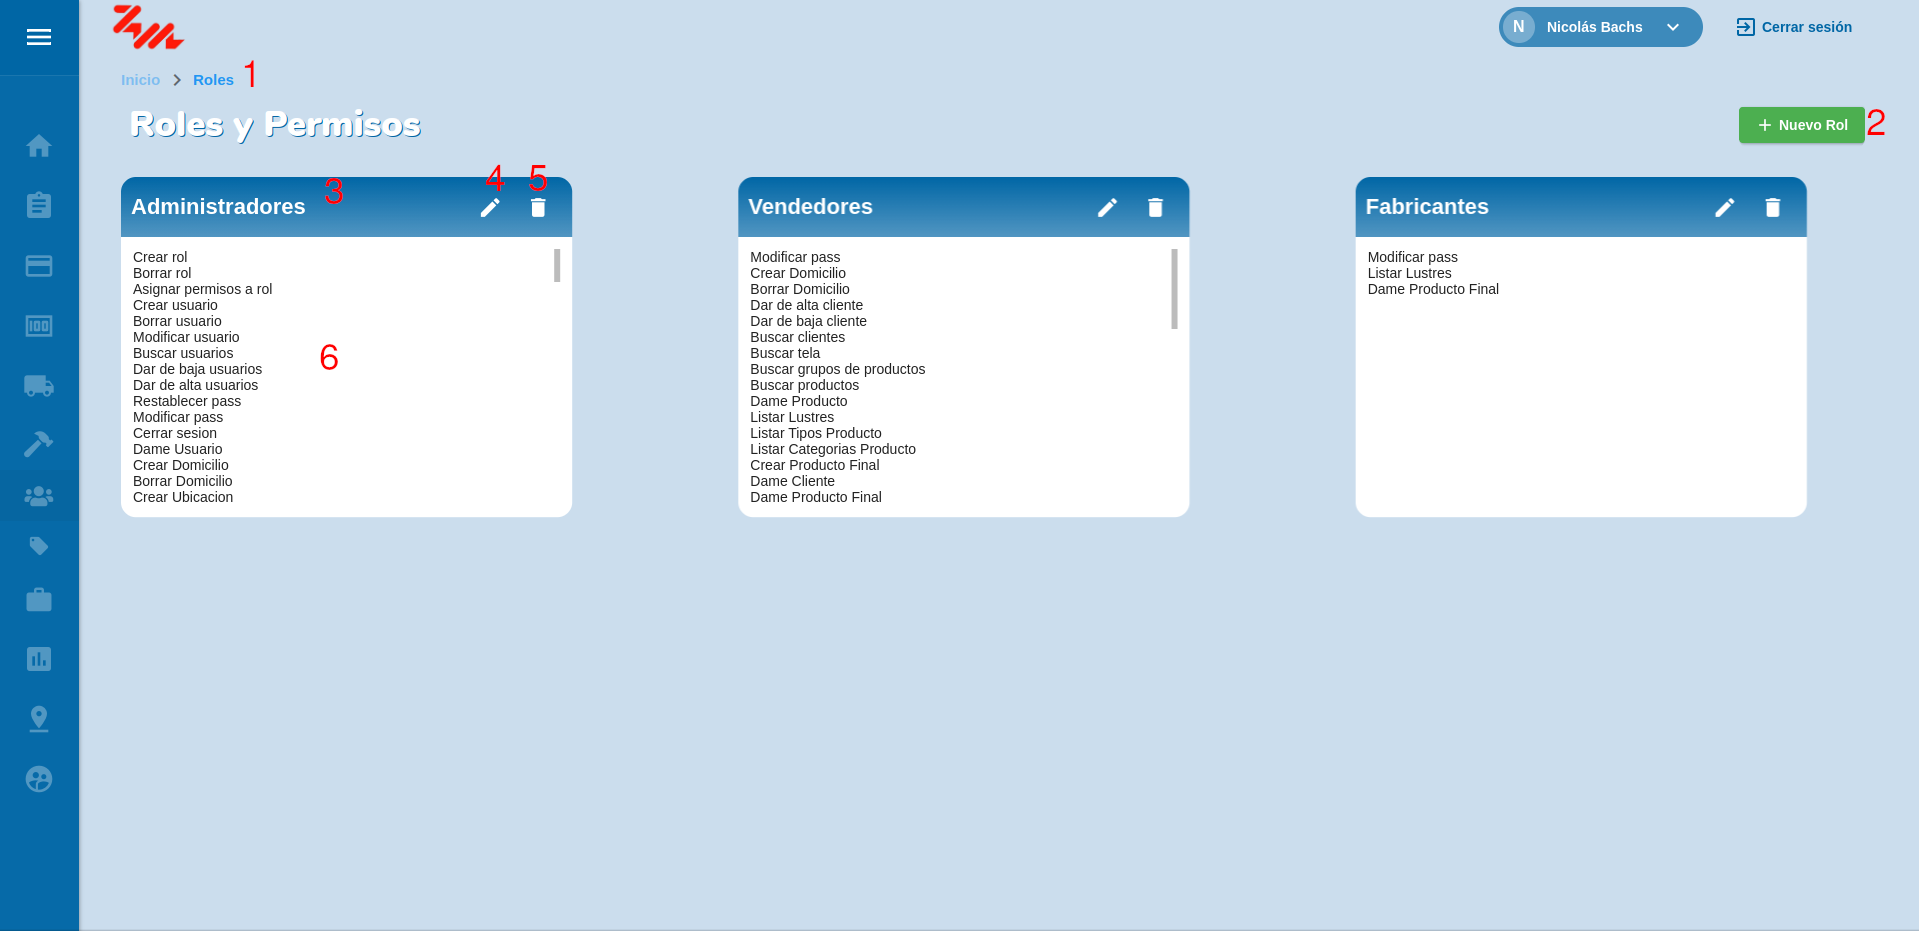
\includegraphics[width=\textwidth,height=\textheight,keepaspectratio]{Escenarios/AD-35-00}
\caption{Escenario - AD-35-00}
\label{fig:AD-35-00}
\end{figure}

Este escenario permite a los usuarios visualizar los distintos roles existenes, los permisos con los que cuenta cada uno de ellos y las acciones que se pueden realizar sobre los mismos.
Con el botón \textbf{AD-35-01} se podrá navegar al escenario \textbf{AD-02-00}. El botón \textbf{AD-35-02} permite crear un nuevo rol, navegando al escenario \textbf{AD-36-00}. Además se muestran los distintos roles, en \textbf{AD-35-03} podemos ver el nombre de uno de esos roles. Con el botón \textbf{AD-35-04} podemos editar el rol, navegando al escenario \textbf{AD-36-00} y con el botón \textbf{AD-35-05} se puede eliminar el rol. En \textbf{AD-35-06} se listan los permisos que tiene asignado el rol.
\clearpage
